\documentclass[1p]{elsarticle_modified}
%\bibliographystyle{elsarticle-num}

%\usepackage[colorlinks]{hyperref}
%\usepackage{abbrmath_seonhwa} %\Abb, \Ascr, \Acal ,\Abf, \Afrak
\usepackage{amsfonts}
\usepackage{amssymb}
\usepackage{amsmath}
\usepackage{amsthm}
\usepackage{scalefnt}
\usepackage{amsbsy}
\usepackage{kotex}
\usepackage{caption}
\usepackage{subfig}
\usepackage{color}
\usepackage{graphicx}
\usepackage{xcolor} %% white, black, red, green, blue, cyan, magenta, yellow
\usepackage{float}
\usepackage{setspace}
\usepackage{hyperref}

\usepackage{tikz}
\usetikzlibrary{arrows}

\usepackage{multirow}
\usepackage{array} % fixed length table
\usepackage{hhline}

%%%%%%%%%%%%%%%%%%%%%
\makeatletter
\renewcommand*\env@matrix[1][\arraystretch]{%
	\edef\arraystretch{#1}%
	\hskip -\arraycolsep
	\let\@ifnextchar\new@ifnextchar
	\array{*\c@MaxMatrixCols c}}
\makeatother %https://tex.stackexchange.com/questions/14071/how-can-i-increase-the-line-spacing-in-a-matrix
%%%%%%%%%%%%%%%

\usepackage[normalem]{ulem}

\newcommand{\msout}[1]{\ifmmode\text{\sout{\ensuremath{#1}}}\else\sout{#1}\fi}
%SOURCE: \msout is \stkout macro in https://tex.stackexchange.com/questions/20609/strikeout-in-math-mode

\newcommand{\cancel}[1]{
	\ifmmode
	{\color{red}\msout{#1}}
	\else
	{\color{red}\sout{#1}}
	\fi
}

\newcommand{\add}[1]{
	{\color{blue}\uwave{#1}}
}

\newcommand{\replace}[2]{
	\ifmmode
	{\color{red}\msout{#1}}{\color{blue}\uwave{#2}}
	\else
	{\color{red}\sout{#1}}{\color{blue}\uwave{#2}}
	\fi
}

\newcommand{\Sol}{\mathcal{S}} %segment
\newcommand{\D}{D} %diagram
\newcommand{\A}{\mathcal{A}} %arc


%%%%%%%%%%%%%%%%%%%%%%%%%%%%%5 test

\def\sl{\operatorname{\textup{SL}}(2,\Cbb)}
\def\psl{\operatorname{\textup{PSL}}(2,\Cbb)}
\def\quan{\mkern 1mu \triangleright \mkern 1mu}

\theoremstyle{definition}
\newtheorem{thm}{Theorem}[section]
\newtheorem{prop}[thm]{Proposition}
\newtheorem{lem}[thm]{Lemma}
\newtheorem{ques}[thm]{Question}
\newtheorem{cor}[thm]{Corollary}
\newtheorem{defn}[thm]{Definition}
\newtheorem{exam}[thm]{Example}
\newtheorem{rmk}[thm]{Remark}
\newtheorem{alg}[thm]{Algorithm}

\newcommand{\I}{\sqrt{-1}}
\begin{document}

%\begin{frontmatter}
%
%\title{Boundary parabolic representations of knots up to 8 crossings}
%
%%% Group authors per affiliation:
%\author{Yunhi Cho} 
%\address{Department of Mathematics, University of Seoul, Seoul, Korea}
%\ead{yhcho@uos.ac.kr}
%
%
%\author{Seonhwa Kim} %\fnref{s_kim}}
%\address{Center for Geometry and Physics, Institute for Basic Science, Pohang, 37673, Korea}
%\ead{ryeona17@ibs.re.kr}
%
%\author{Hyuk Kim}
%\address{Department of Mathematical Sciences, Seoul National University, Seoul 08826, Korea}
%\ead{hyukkim@snu.ac.kr}
%
%\author{Seokbeom Yoon}
%\address{Department of Mathematical Sciences, Seoul National University, Seoul, 08826,  Korea}
%\ead{sbyoon15@snu.ac.kr}
%
%\begin{abstract}
%We find all boundary parabolic representation of knots up to 8 crossings.
%
%\end{abstract}
%\begin{keyword}
%    \MSC[2010] 57M25 
%\end{keyword}
%
%\end{frontmatter}

%\linenumbers
%\tableofcontents
%
\newcommand\colored[1]{\textcolor{white}{\rule[-0.35ex]{0.8em}{1.4ex}}\kern-0.8em\color{red} #1}%
%\newcommand\colored[1]{\textcolor{white}{ #1}\kern-2.17ex	\textcolor{white}{ #1}\kern-1.81ex	\textcolor{white}{ #1}\kern-2.15ex\color{red}#1	}

{\Large $\underline{12a_{0370}~(K12a_{0370})}$}

\setlength{\tabcolsep}{10pt}
\renewcommand{\arraystretch}{1.6}
\vspace{1cm}\begin{tabular}{m{100pt}>{\centering\arraybackslash}m{274pt}}
\multirow{5}{120pt}{
	\centering
	\includegraphics[width=112pt]{../../../GIT/diagram.site/Diagrams/png/1171_12a_0370.png}\\
\ \ \ A knot diagram\footnotemark}&
\allowdisplaybreaks
\textbf{Linearized knot diagam} \\
\cline{2-2}
 &
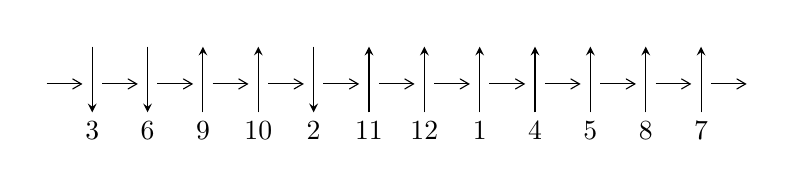
\begin{tikzpicture}[x=20pt, y=17pt]
	% nodes
	\node (C0) at (0, 0) {};
	\node (C1) at (1, 0) {};
	\node (C1U) at (1, +1) {};
	\node (C1D) at (1, -1) {3};

	\node (C2) at (2, 0) {};
	\node (C2U) at (2, +1) {};
	\node (C2D) at (2, -1) {6};

	\node (C3) at (3, 0) {};
	\node (C3U) at (3, +1) {};
	\node (C3D) at (3, -1) {9};

	\node (C4) at (4, 0) {};
	\node (C4U) at (4, +1) {};
	\node (C4D) at (4, -1) {10};

	\node (C5) at (5, 0) {};
	\node (C5U) at (5, +1) {};
	\node (C5D) at (5, -1) {2};

	\node (C6) at (6, 0) {};
	\node (C6U) at (6, +1) {};
	\node (C6D) at (6, -1) {11};

	\node (C7) at (7, 0) {};
	\node (C7U) at (7, +1) {};
	\node (C7D) at (7, -1) {12};

	\node (C8) at (8, 0) {};
	\node (C8U) at (8, +1) {};
	\node (C8D) at (8, -1) {1};

	\node (C9) at (9, 0) {};
	\node (C9U) at (9, +1) {};
	\node (C9D) at (9, -1) {4};

	\node (C10) at (10, 0) {};
	\node (C10U) at (10, +1) {};
	\node (C10D) at (10, -1) {5};

	\node (C11) at (11, 0) {};
	\node (C11U) at (11, +1) {};
	\node (C11D) at (11, -1) {8};

	\node (C12) at (12, 0) {};
	\node (C12U) at (12, +1) {};
	\node (C12D) at (12, -1) {7};
	\node (C13) at (13, 0) {};

	% arrows
	\draw[->,>={angle 60}]
	(C0) edge (C1) (C1) edge (C2) (C2) edge (C3) (C3) edge (C4) (C4) edge (C5) (C5) edge (C6) (C6) edge (C7) (C7) edge (C8) (C8) edge (C9) (C9) edge (C10) (C10) edge (C11) (C11) edge (C12) (C12) edge (C13) ;	\draw[->,>=stealth]
	(C1U) edge (C1D) (C2U) edge (C2D) (C3D) edge (C3U) (C4D) edge (C4U) (C5U) edge (C5D) (C6D) edge (C6U) (C7D) edge (C7U) (C8D) edge (C8U) (C9D) edge (C9U) (C10D) edge (C10U) (C11D) edge (C11U) (C12D) edge (C12U) ;
	\end{tikzpicture} \\
\hhline{~~} \\& 
\textbf{Solving Sequence} \\ \cline{2-2} 
 &
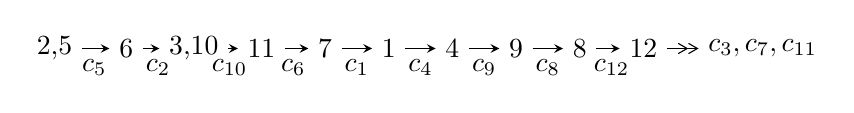
\begin{tikzpicture}[x=23pt, y=7pt]
	% node
	\node (A0) at (-1/8, 0) {2,5};
	\node (A1) at (1, 0) {6};
	\node (A2) at (33/16, 0) {3,10};
	\node (A3) at (25/8, 0) {11};
	\node (A4) at (33/8, 0) {7};
	\node (A5) at (41/8, 0) {1};
	\node (A6) at (49/8, 0) {4};
	\node (A7) at (57/8, 0) {9};
	\node (A8) at (65/8, 0) {8};
	\node (A9) at (73/8, 0) {12};
	\node (C1) at (1/2, -1) {$c_{5}$};
	\node (C2) at (3/2, -1) {$c_{2}$};
	\node (C3) at (21/8, -1) {$c_{10}$};
	\node (C4) at (29/8, -1) {$c_{6}$};
	\node (C5) at (37/8, -1) {$c_{1}$};
	\node (C6) at (45/8, -1) {$c_{4}$};
	\node (C7) at (53/8, -1) {$c_{9}$};
	\node (C8) at (61/8, -1) {$c_{8}$};
	\node (C9) at (69/8, -1) {$c_{12}$};
	\node (A10) at (11, 0) {$c_{3},c_{7},c_{11}$};

	% edge
	\draw[->,>=stealth]	
	(A0) edge (A1) (A1) edge (A2) (A2) edge (A3) (A3) edge (A4) (A4) edge (A5) (A5) edge (A6) (A6) edge (A7) (A7) edge (A8) (A8) edge (A9) ;
	\draw[->>,>={angle 60}]	
	(A9) edge (A10);
\end{tikzpicture} \\ 

\end{tabular} \\

\footnotetext{
The image of knot diagram is generated by the software ``\textbf{Draw programme}" developed by Andrew Bartholomew(\url{http://www.layer8.co.uk/maths/draw/index.htm\#Running-draw}), where we modified some parts for our purpose(\url{https://github.com/CATsTAILs/LinksPainter}).
}\phantom \\ \newline 
\centering \textbf{Ideals for irreducible components\footnotemark of $X_{\text{par}}$} 
 
\begin{align*}
I^u_{1}&=\langle 
1.57162\times10^{65} u^{64}+6.57175\times10^{65} u^{63}+\cdots+2.92397\times10^{65} b-2.95547\times10^{66},\\
\phantom{I^u_{1}}&\phantom{= \langle  }1.26210\times10^{66} u^{64}+4.50966\times10^{66} u^{63}+\cdots+4.09356\times10^{66} a-1.01879\times10^{67},\;u^{65}+4 u^{64}+\cdots-51 u+7\rangle \\
I^u_{2}&=\langle 
b,\;a^3+a^2-1,\;u+1\rangle \\
I^u_{3}&=\langle 
b^2-2,\;a^3- a^2+1,\;u-1\rangle \\
\\
\end{align*}
\raggedright * 3 irreducible components of $\dim_{\mathbb{C}}=0$, with total 74 representations.\\
\footnotetext{All coefficients of polynomials are rational numbers. But the coefficients are sometimes approximated in decimal forms when there is not enough margin.}
\newpage
\renewcommand{\arraystretch}{1}
\centering \section*{I. $I^u_{1}= \langle 1.57\times10^{65} u^{64}+6.57\times10^{65} u^{63}+\cdots+2.92\times10^{65} b-2.96\times10^{66},\;1.26\times10^{66} u^{64}+4.51\times10^{66} u^{63}+\cdots+4.09\times10^{66} a-1.02\times10^{67},\;u^{65}+4 u^{64}+\cdots-51 u+7 \rangle$}
\flushleft \textbf{(i) Arc colorings}\\
\begin{tabular}{m{7pt} m{180pt} m{7pt} m{180pt} }
\flushright $a_{2}=$&$\begin{pmatrix}0\\u\end{pmatrix}$ \\
\flushright $a_{5}=$&$\begin{pmatrix}1\\0\end{pmatrix}$ \\
\flushright $a_{6}=$&$\begin{pmatrix}1\\u^2\end{pmatrix}$ \\
\flushright $a_{3}=$&$\begin{pmatrix}- u\\- u^3+u\end{pmatrix}$ \\
\flushright $a_{10}=$&$\begin{pmatrix}-0.308313 u^{64}-1.10165 u^{63}+\cdots-26.1352 u+2.48875\\-0.537494 u^{64}-2.24754 u^{63}+\cdots-43.5603 u+10.1077\end{pmatrix}$ \\
\flushright $a_{11}=$&$\begin{pmatrix}-0.845807 u^{64}-3.34919 u^{63}+\cdots-69.6955 u+12.5965\\-0.537494 u^{64}-2.24754 u^{63}+\cdots-43.5603 u+10.1077\end{pmatrix}$ \\
\flushright $a_{7}=$&$\begin{pmatrix}-0.896834 u^{64}-4.06581 u^{63}+\cdots-104.086 u+24.6201\\-0.334251 u^{64}-1.33325 u^{63}+\cdots-27.2815 u+5.97496\end{pmatrix}$ \\
\flushright $a_{1}=$&$\begin{pmatrix}u^3\\u^5- u^3+u\end{pmatrix}$ \\
\flushright $a_{4}=$&$\begin{pmatrix}0.938529 u^{64}+4.21121 u^{63}+\cdots+83.4299 u-19.2445\\0.427727 u^{64}+1.79587 u^{63}+\cdots+45.3628 u-9.76939\end{pmatrix}$ \\
\flushright $a_{9}=$&$\begin{pmatrix}1.57556 u^{64}+6.38013 u^{63}+\cdots+112.041 u-27.9236\\0.190879 u^{64}+1.27293 u^{63}+\cdots+6.17774 u-2.70329\end{pmatrix}$ \\
\flushright $a_{8}=$&$\begin{pmatrix}1.20468 u^{64}+5.47814 u^{63}+\cdots+111.316 u-28.2011\\0.371889 u^{64}+1.74141 u^{63}+\cdots+25.4181 u-6.03071\end{pmatrix}$ \\
\flushright $a_{12}=$&$\begin{pmatrix}-0.221510 u^{64}-0.993540 u^{63}+\cdots-40.1704 u+6.43709\\-0.326133 u^{64}-1.36825 u^{63}+\cdots-16.1337 u+4.29430\end{pmatrix}$\\&\end{tabular}
\flushleft \textbf{(ii) Obstruction class $= -1$}\\~\\
\flushleft \textbf{(iii) Cusp Shapes $= 0.860917 u^{64}+3.71890 u^{63}+\cdots+8.19845 u+13.2317$}\\~\\
\newpage\renewcommand{\arraystretch}{1}
\flushleft \textbf{(iv) u-Polynomials at the component}\newline \\
\begin{tabular}{m{50pt}|m{274pt}}
Crossings & \hspace{64pt}u-Polynomials at each crossing \\
\hline $$\begin{aligned}c_{1}\end{aligned}$$&$\begin{aligned}
&u^{65}+28 u^{64}+\cdots+1621 u+49
\end{aligned}$\\
\hline $$\begin{aligned}c_{2},c_{5}\end{aligned}$$&$\begin{aligned}
&u^{65}+4 u^{64}+\cdots-51 u+7
\end{aligned}$\\
\hline $$\begin{aligned}c_{3},c_{4},c_{9}\\c_{10}\end{aligned}$$&$\begin{aligned}
&u^{65}- u^{64}+\cdots-8 u-8
\end{aligned}$\\
\hline $$\begin{aligned}c_{6},c_{8}\end{aligned}$$&$\begin{aligned}
&u^{65}+2 u^{64}+\cdots+2788 u+289
\end{aligned}$\\
\hline $$\begin{aligned}c_{7},c_{11},c_{12}\end{aligned}$$&$\begin{aligned}
&u^{65}-2 u^{64}+\cdots+8 u+1
\end{aligned}$\\
\hline
\end{tabular}\\~\\
\newpage\renewcommand{\arraystretch}{1}
\flushleft \textbf{(v) Riley Polynomials at the component}\newline \\
\begin{tabular}{m{50pt}|m{274pt}}
Crossings & \hspace{64pt}Riley Polynomials at each crossing \\
\hline $$\begin{aligned}c_{1}\end{aligned}$$&$\begin{aligned}
&y^{65}+28 y^{64}+\cdots+644709 y-2401
\end{aligned}$\\
\hline $$\begin{aligned}c_{2},c_{5}\end{aligned}$$&$\begin{aligned}
&y^{65}-28 y^{64}+\cdots+1621 y-49
\end{aligned}$\\
\hline $$\begin{aligned}c_{3},c_{4},c_{9}\\c_{10}\end{aligned}$$&$\begin{aligned}
&y^{65}-79 y^{64}+\cdots+1728 y-64
\end{aligned}$\\
\hline $$\begin{aligned}c_{6},c_{8}\end{aligned}$$&$\begin{aligned}
&y^{65}-50 y^{64}+\cdots+7602434 y-83521
\end{aligned}$\\
\hline $$\begin{aligned}c_{7},c_{11},c_{12}\end{aligned}$$&$\begin{aligned}
&y^{65}+54 y^{64}+\cdots+98 y-1
\end{aligned}$\\
\hline
\end{tabular}\\~\\
\newpage\flushleft \textbf{(vi) Complex Volumes and Cusp Shapes}
$$\begin{array}{c|c|c}  
\text{Solutions to }I^u_{1}& \I (\text{vol} + \sqrt{-1}CS) & \text{Cusp shape}\\
 \hline 
\begin{aligned}
u &= \phantom{-}0.612176 + 0.789701 I \\
a &= \phantom{-}0.561126 + 0.096922 I \\
b &= -0.952670 - 0.404352 I\end{aligned}
 & \phantom{-}6.34514 + 1.30632 I & \phantom{-}13.77211 - 1.31410 I \\ \hline\begin{aligned}
u &= \phantom{-}0.612176 - 0.789701 I \\
a &= \phantom{-}0.561126 - 0.096922 I \\
b &= -0.952670 + 0.404352 I\end{aligned}
 & \phantom{-}6.34514 - 1.30632 I & \phantom{-}13.77211 + 1.31410 I \\ \hline\begin{aligned}
u &= -0.747787 + 0.667407 I \\
a &= -0.360811 + 0.449280 I \\
b &= -0.034903 + 0.726729 I\end{aligned}
 & -0.65467 - 1.56191 I & \phantom{-}6.00000 + 0. I\phantom{ +0.000000I} \\ \hline\begin{aligned}
u &= -0.747787 - 0.667407 I \\
a &= -0.360811 - 0.449280 I \\
b &= -0.034903 - 0.726729 I\end{aligned}
 & -0.65467 + 1.56191 I & \phantom{-}6.00000 + 0. I\phantom{ +0.000000I} \\ \hline\begin{aligned}
u &= \phantom{-}0.537868 + 0.834733 I \\
a &= -0.578993 - 0.033369 I \\
b &= \phantom{-}0.891890 + 0.462986 I\end{aligned}
 & \phantom{-}2.20984 + 5.53743 I & \phantom{-}9.36866 - 4.50579 I \\ \hline\begin{aligned}
u &= \phantom{-}0.537868 - 0.834733 I \\
a &= -0.578993 + 0.033369 I \\
b &= \phantom{-}0.891890 - 0.462986 I\end{aligned}
 & \phantom{-}2.20984 - 5.53743 I & \phantom{-}9.36866 + 4.50579 I \\ \hline\begin{aligned}
u &= \phantom{-}0.879407 + 0.497658 I \\
a &= \phantom{-}1.025300 + 0.888790 I \\
b &= -0.712730 + 0.316213 I\end{aligned}
 & \phantom{-}0.21641 - 3.44473 I & \phantom{-}7.87016 + 8.48336 I \\ \hline\begin{aligned}
u &= \phantom{-}0.879407 - 0.497658 I \\
a &= \phantom{-}1.025300 - 0.888790 I \\
b &= -0.712730 - 0.316213 I\end{aligned}
 & \phantom{-}0.21641 + 3.44473 I & \phantom{-}7.87016 - 8.48336 I \\ \hline\begin{aligned}
u &= \phantom{-}0.698155 + 0.733599 I \\
a &= -0.513257 - 0.173198 I \\
b &= \phantom{-}1.036060 + 0.336652 I\end{aligned}
 & \phantom{-}2.63490 - 2.89952 I & \phantom{-}9.88169 + 2.65135 I \\ \hline\begin{aligned}
u &= \phantom{-}0.698155 - 0.733599 I \\
a &= -0.513257 + 0.173198 I \\
b &= \phantom{-}1.036060 - 0.336652 I\end{aligned}
 & \phantom{-}2.63490 + 2.89952 I & \phantom{-}9.88169 - 2.65135 I\\
 \hline 
 \end{array}$$\newpage$$\begin{array}{c|c|c}  
\text{Solutions to }I^u_{1}& \I (\text{vol} + \sqrt{-1}CS) & \text{Cusp shape}\\
 \hline 
\begin{aligned}
u &= \phantom{-}1.04736\phantom{ +0.000000I} \\
a &= -0.0308709\phantom{ +0.000000I} \\
b &= \phantom{-}1.43162\phantom{ +0.000000I}\end{aligned}
 & \phantom{-}3.32536\phantom{ +0.000000I} & \phantom{-}1.90800\phantom{ +0.000000I} \\ \hline\begin{aligned}
u &= -0.688518 + 0.611372 I \\
a &= -2.95116 + 0.90249 I \\
b &= \phantom{-}1.56873 + 0.00323 I\end{aligned}
 & \phantom{-}2.81749 - 1.96826 I & \phantom{-}8.01195 + 0.26172 I \\ \hline\begin{aligned}
u &= -0.688518 - 0.611372 I \\
a &= -2.95116 - 0.90249 I \\
b &= \phantom{-}1.56873 - 0.00323 I\end{aligned}
 & \phantom{-}2.81749 + 1.96826 I & \phantom{-}8.01195 - 0.26172 I \\ \hline\begin{aligned}
u &= -0.859363 + 0.654709 I \\
a &= \phantom{-}0.345067 - 0.440186 I \\
b &= \phantom{-}0.113262 - 0.740531 I\end{aligned}
 & \phantom{-}2.97311 + 2.54501 I & \phantom{-0.000000 } 0 \\ \hline\begin{aligned}
u &= -0.859363 - 0.654709 I \\
a &= \phantom{-}0.345067 + 0.440186 I \\
b &= \phantom{-}0.113262 + 0.740531 I\end{aligned}
 & \phantom{-}2.97311 - 2.54501 I & \phantom{-0.000000 } 0 \\ \hline\begin{aligned}
u &= -0.792220 + 0.742732 I \\
a &= \phantom{-}2.28438 - 0.98600 I \\
b &= -1.61762 - 0.02352 I\end{aligned}
 & \phantom{-}8.72128 + 0.76781 I & \phantom{-0.000000 } 0 \\ \hline\begin{aligned}
u &= -0.792220 - 0.742732 I \\
a &= \phantom{-}2.28438 + 0.98600 I \\
b &= -1.61762 + 0.02352 I\end{aligned}
 & \phantom{-}8.72128 - 0.76781 I & \phantom{-0.000000 } 0 \\ \hline\begin{aligned}
u &= -0.879226 + 0.208718 I \\
a &= -0.212799 + 0.396317 I \\
b &= -0.139382 + 0.414404 I\end{aligned}
 & -1.47345 + 0.81303 I & -1.06179 - 2.21079 I \\ \hline\begin{aligned}
u &= -0.879226 - 0.208718 I \\
a &= -0.212799 - 0.396317 I \\
b &= -0.139382 - 0.414404 I\end{aligned}
 & -1.47345 - 0.81303 I & -1.06179 + 2.21079 I \\ \hline\begin{aligned}
u &= \phantom{-}1.018090 + 0.446326 I \\
a &= -1.00410 - 1.10254 I \\
b &= \phantom{-}0.594982 - 0.430810 I\end{aligned}
 & -5.61394 - 4.98473 I & \phantom{-0.000000 } 0\\
 \hline 
 \end{array}$$\newpage$$\begin{array}{c|c|c}  
\text{Solutions to }I^u_{1}& \I (\text{vol} + \sqrt{-1}CS) & \text{Cusp shape}\\
 \hline 
\begin{aligned}
u &= \phantom{-}1.018090 - 0.446326 I \\
a &= -1.00410 + 1.10254 I \\
b &= \phantom{-}0.594982 + 0.430810 I\end{aligned}
 & -5.61394 + 4.98473 I & \phantom{-0.000000 } 0 \\ \hline\begin{aligned}
u &= -1.090720 + 0.327345 I \\
a &= \phantom{-}0.346639 - 0.382185 I \\
b &= \phantom{-}0.354858 - 0.503499 I\end{aligned}
 & -6.33395 + 1.70228 I & \phantom{-0.000000 } 0 \\ \hline\begin{aligned}
u &= -1.090720 - 0.327345 I \\
a &= \phantom{-}0.346639 + 0.382185 I \\
b &= \phantom{-}0.354858 + 0.503499 I\end{aligned}
 & -6.33395 - 1.70228 I & \phantom{-0.000000 } 0 \\ \hline\begin{aligned}
u &= \phantom{-}0.835134 + 0.207071 I \\
a &= \phantom{-}1.74135 + 0.81734 I \\
b &= -0.458541 + 0.146079 I\end{aligned}
 & -4.20314 + 2.29651 I & \phantom{-}7.92045 + 3.19787 I \\ \hline\begin{aligned}
u &= \phantom{-}0.835134 - 0.207071 I \\
a &= \phantom{-}1.74135 - 0.81734 I \\
b &= -0.458541 - 0.146079 I\end{aligned}
 & -4.20314 - 2.29651 I & \phantom{-}7.92045 - 3.19787 I \\ \hline\begin{aligned}
u &= -0.942425 + 0.650639 I \\
a &= -0.339182 + 0.434920 I \\
b &= -0.173665 + 0.754967 I\end{aligned}
 & -1.25054 + 6.68721 I & \phantom{-0.000000 } 0 \\ \hline\begin{aligned}
u &= -0.942425 - 0.650639 I \\
a &= -0.339182 - 0.434920 I \\
b &= -0.173665 - 0.754967 I\end{aligned}
 & -1.25054 - 6.68721 I & \phantom{-0.000000 } 0 \\ \hline\begin{aligned}
u &= -0.477249 + 1.048800 I \\
a &= \phantom{-}1.83392 - 0.00459 I \\
b &= -1.66803 + 0.12607 I\end{aligned}
 & \phantom{-}11.03680 - 7.80758 I & \phantom{-0.000000 } 0 \\ \hline\begin{aligned}
u &= -0.477249 - 1.048800 I \\
a &= \phantom{-}1.83392 + 0.00459 I \\
b &= -1.66803 - 0.12607 I\end{aligned}
 & \phantom{-}11.03680 + 7.80758 I & \phantom{-0.000000 } 0 \\ \hline\begin{aligned}
u &= \phantom{-}1.121100 + 0.284148 I \\
a &= \phantom{-}0.127434 + 0.111845 I \\
b &= -1.44392 - 0.12372 I\end{aligned}
 & -0.503562 + 0.442865 I & \phantom{-0.000000 } 0\\
 \hline 
 \end{array}$$\newpage$$\begin{array}{c|c|c}  
\text{Solutions to }I^u_{1}& \I (\text{vol} + \sqrt{-1}CS) & \text{Cusp shape}\\
 \hline 
\begin{aligned}
u &= \phantom{-}1.121100 - 0.284148 I \\
a &= \phantom{-}0.127434 - 0.111845 I \\
b &= -1.44392 + 0.12372 I\end{aligned}
 & -0.503562 - 0.442865 I & \phantom{-0.000000 } 0 \\ \hline\begin{aligned}
u &= -0.542642 + 1.041680 I \\
a &= -1.84192 + 0.12408 I \\
b &= \phantom{-}1.67890 - 0.10309 I\end{aligned}
 & \phantom{-}15.4602 - 3.2500 I & \phantom{-0.000000 } 0 \\ \hline\begin{aligned}
u &= -0.542642 - 1.041680 I \\
a &= -1.84192 - 0.12408 I \\
b &= \phantom{-}1.67890 + 0.10309 I\end{aligned}
 & \phantom{-}15.4602 + 3.2500 I & \phantom{-0.000000 } 0 \\ \hline\begin{aligned}
u &= -1.000100 + 0.618281 I \\
a &= \phantom{-}1.89737 - 1.82085 I \\
b &= -1.58542 - 0.10501 I\end{aligned}
 & \phantom{-}1.82316 + 6.85461 I & \phantom{-0.000000 } 0 \\ \hline\begin{aligned}
u &= -1.000100 - 0.618281 I \\
a &= \phantom{-}1.89737 + 1.82085 I \\
b &= -1.58542 + 0.10501 I\end{aligned}
 & \phantom{-}1.82316 - 6.85461 I & \phantom{-0.000000 } 0 \\ \hline\begin{aligned}
u &= -0.929923 + 0.728312 I \\
a &= -1.97076 + 1.33085 I \\
b &= \phantom{-}1.62385 + 0.07311 I\end{aligned}
 & \phantom{-}8.30513 + 4.82290 I & \phantom{-0.000000 } 0 \\ \hline\begin{aligned}
u &= -0.929923 - 0.728312 I \\
a &= -1.97076 - 1.33085 I \\
b &= \phantom{-}1.62385 - 0.07311 I\end{aligned}
 & \phantom{-}8.30513 - 4.82290 I & \phantom{-0.000000 } 0 \\ \hline\begin{aligned}
u &= \phantom{-}0.716718 + 0.381500 I \\
a &= -1.220570 - 0.577631 I \\
b &= \phantom{-}0.643611 - 0.098429 I\end{aligned}
 & \phantom{-}0.785742 - 0.346166 I & \phantom{-}11.27090 + 0.19465 I \\ \hline\begin{aligned}
u &= \phantom{-}0.716718 - 0.381500 I \\
a &= -1.220570 + 0.577631 I \\
b &= \phantom{-}0.643611 + 0.098429 I\end{aligned}
 & \phantom{-}0.785742 + 0.346166 I & \phantom{-}11.27090 - 0.19465 I \\ \hline\begin{aligned}
u &= -0.616760 + 1.016660 I \\
a &= \phantom{-}1.86366 - 0.26965 I \\
b &= -1.68444 + 0.07351 I\end{aligned}
 & \phantom{-}12.05520 + 1.42142 I & \phantom{-0.000000 } 0\\
 \hline 
 \end{array}$$\newpage$$\begin{array}{c|c|c}  
\text{Solutions to }I^u_{1}& \I (\text{vol} + \sqrt{-1}CS) & \text{Cusp shape}\\
 \hline 
\begin{aligned}
u &= -0.616760 - 1.016660 I \\
a &= \phantom{-}1.86366 + 0.26965 I \\
b &= -1.68444 - 0.07351 I\end{aligned}
 & \phantom{-}12.05520 - 1.42142 I & \phantom{-0.000000 } 0 \\ \hline\begin{aligned}
u &= \phantom{-}0.965461 + 0.702359 I \\
a &= \phantom{-}0.835684 + 0.911173 I \\
b &= -0.858855 + 0.509945 I\end{aligned}
 & \phantom{-}1.85518 - 2.58936 I & \phantom{-0.000000 } 0 \\ \hline\begin{aligned}
u &= \phantom{-}0.965461 - 0.702359 I \\
a &= \phantom{-}0.835684 - 0.911173 I \\
b &= -0.858855 - 0.509945 I\end{aligned}
 & \phantom{-}1.85518 + 2.58936 I & \phantom{-0.000000 } 0 \\ \hline\begin{aligned}
u &= -1.19939\phantom{ +0.000000I} \\
a &= \phantom{-}0.542136\phantom{ +0.000000I} \\
b &= \phantom{-}0.558137\phantom{ +0.000000I}\end{aligned}
 & \phantom{-}0.215305\phantom{ +0.000000I} & \phantom{-0.000000 } 0 \\ \hline\begin{aligned}
u &= -1.223990 + 0.070272 I \\
a &= -0.568813 + 0.167355 I \\
b &= -0.598816 + 0.153922 I\end{aligned}
 & -3.79500 - 3.51729 I & \phantom{-0.000000 } 0 \\ \hline\begin{aligned}
u &= -1.223990 - 0.070272 I \\
a &= -0.568813 - 0.167355 I \\
b &= -0.598816 - 0.153922 I\end{aligned}
 & -3.79500 + 3.51729 I & \phantom{-0.000000 } 0 \\ \hline\begin{aligned}
u &= \phantom{-}1.036490 + 0.697733 I \\
a &= -0.809759 - 0.942093 I \\
b &= \phantom{-}0.818309 - 0.567364 I\end{aligned}
 & \phantom{-}5.09312 - 6.92778 I & \phantom{-0.000000 } 0 \\ \hline\begin{aligned}
u &= \phantom{-}1.036490 - 0.697733 I \\
a &= -0.809759 + 0.942093 I \\
b &= \phantom{-}0.818309 + 0.567364 I\end{aligned}
 & \phantom{-}5.09312 + 6.92778 I & \phantom{-0.000000 } 0 \\ \hline\begin{aligned}
u &= \phantom{-}1.084460 + 0.684896 I \\
a &= \phantom{-}0.789764 + 0.966569 I \\
b &= -0.784743 + 0.601883 I\end{aligned}
 & \phantom{-}0.58292 - 11.22380 I & \phantom{-0.000000 } 0 \\ \hline\begin{aligned}
u &= \phantom{-}1.084460 - 0.684896 I \\
a &= \phantom{-}0.789764 - 0.966569 I \\
b &= -0.784743 - 0.601883 I\end{aligned}
 & \phantom{-}0.58292 + 11.22380 I & \phantom{-0.000000 } 0\\
 \hline 
 \end{array}$$\newpage$$\begin{array}{c|c|c}  
\text{Solutions to }I^u_{1}& \I (\text{vol} + \sqrt{-1}CS) & \text{Cusp shape}\\
 \hline 
\begin{aligned}
u &= -1.113940 + 0.786858 I \\
a &= -1.41064 + 1.35680 I \\
b &= \phantom{-}1.66142 + 0.14314 I\end{aligned}
 & \phantom{-}10.51140 + 5.10195 I & \phantom{-0.000000 } 0 \\ \hline\begin{aligned}
u &= -1.113940 - 0.786858 I \\
a &= -1.41064 - 1.35680 I \\
b &= \phantom{-}1.66142 - 0.14314 I\end{aligned}
 & \phantom{-}10.51140 - 5.10195 I & \phantom{-0.000000 } 0 \\ \hline\begin{aligned}
u &= -1.163830 + 0.759847 I \\
a &= \phantom{-}1.29115 - 1.43417 I \\
b &= -1.65344 - 0.16744 I\end{aligned}
 & \phantom{-}13.5310 + 9.7563 I & \phantom{-0.000000 } 0 \\ \hline\begin{aligned}
u &= -1.163830 - 0.759847 I \\
a &= \phantom{-}1.29115 + 1.43417 I \\
b &= -1.65344 + 0.16744 I\end{aligned}
 & \phantom{-}13.5310 - 9.7563 I & \phantom{-0.000000 } 0 \\ \hline\begin{aligned}
u &= -1.192080 + 0.730572 I \\
a &= -1.21566 + 1.50565 I \\
b &= \phantom{-}1.64210 + 0.18253 I\end{aligned}
 & \phantom{-}8.8189 + 14.2263 I & \phantom{-0.000000 } 0 \\ \hline\begin{aligned}
u &= -1.192080 - 0.730572 I \\
a &= -1.21566 - 1.50565 I \\
b &= \phantom{-}1.64210 - 0.18253 I\end{aligned}
 & \phantom{-}8.8189 - 14.2263 I & \phantom{-0.000000 } 0 \\ \hline\begin{aligned}
u &= \phantom{-}1.42411\phantom{ +0.000000I} \\
a &= \phantom{-}0.159460\phantom{ +0.000000I} \\
b &= -1.60305\phantom{ +0.000000I}\end{aligned}
 & \phantom{-}7.84976\phantom{ +0.000000I} & \phantom{-0.000000 } 0 \\ \hline\begin{aligned}
u &= \phantom{-}1.42552 + 0.07021 I \\
a &= -0.161047 - 0.012113 I \\
b &= \phantom{-}1.60335 + 0.03552 I\end{aligned}
 & \phantom{-}3.90623 + 4.17049 I & \phantom{-0.000000 } 0 \\ \hline\begin{aligned}
u &= \phantom{-}1.42552 - 0.07021 I \\
a &= -0.161047 + 0.012113 I \\
b &= \phantom{-}1.60335 - 0.03552 I\end{aligned}
 & \phantom{-}3.90623 - 4.17049 I & \phantom{-0.000000 } 0 \\ \hline\begin{aligned}
u &= \phantom{-}0.012164 + 0.540343 I \\
a &= \phantom{-}0.787036 - 0.425151 I \\
b &= -0.383178 - 0.436316 I\end{aligned}
 & -3.21514 + 1.52290 I & \phantom{-}5.38087 - 4.43310 I\\
 \hline 
 \end{array}$$\newpage$$\begin{array}{c|c|c}  
\text{Solutions to }I^u_{1}& \I (\text{vol} + \sqrt{-1}CS) & \text{Cusp shape}\\
 \hline 
\begin{aligned}
u &= \phantom{-}0.012164 - 0.540343 I \\
a &= \phantom{-}0.787036 + 0.425151 I \\
b &= -0.383178 + 0.436316 I\end{aligned}
 & -3.21514 - 1.52290 I & \phantom{-}5.38087 + 4.43310 I \\ \hline\begin{aligned}
u &= \phantom{-}0.377484 + 0.366802 I \\
a &= \phantom{-}0.07583 - 1.59486 I \\
b &= \phantom{-}1.322440 - 0.065855 I\end{aligned}
 & \phantom{-}2.05865 - 3.23471 I & \phantom{-}10.89405 + 4.40187 I \\ \hline\begin{aligned}
u &= \phantom{-}0.377484 - 0.366802 I \\
a &= \phantom{-}0.07583 + 1.59486 I \\
b &= \phantom{-}1.322440 + 0.065855 I\end{aligned}
 & \phantom{-}2.05865 + 3.23471 I & \phantom{-}10.89405 - 4.40187 I \\ \hline\begin{aligned}
u &= \phantom{-}0.348475\phantom{ +0.000000I} \\
a &= -2.14252\phantom{ +0.000000I} \\
b &= -1.35387\phantom{ +0.000000I}\end{aligned}
 & \phantom{-}5.84839\phantom{ +0.000000I} & \phantom{-}16.9730\phantom{ +0.000000I} \\ \hline\begin{aligned}
u &= \phantom{-}0.260517\phantom{ +0.000000I} \\
a &= -1.67780\phantom{ +0.000000I} \\
b &= \phantom{-}0.360345\phantom{ +0.000000I}\end{aligned}
 & \phantom{-}0.625974\phantom{ +0.000000I} & \phantom{-}16.0870\phantom{ +0.000000I}\\
 \hline 
 \end{array}$$\newpage\newpage\renewcommand{\arraystretch}{1}
\centering \section*{II. $I^u_{2}= \langle b,\;a^3+a^2-1,\;u+1 \rangle$}
\flushleft \textbf{(i) Arc colorings}\\
\begin{tabular}{m{7pt} m{180pt} m{7pt} m{180pt} }
\flushright $a_{2}=$&$\begin{pmatrix}0\\-1\end{pmatrix}$ \\
\flushright $a_{5}=$&$\begin{pmatrix}1\\0\end{pmatrix}$ \\
\flushright $a_{6}=$&$\begin{pmatrix}1\\1\end{pmatrix}$ \\
\flushright $a_{3}=$&$\begin{pmatrix}1\\0\end{pmatrix}$ \\
\flushright $a_{10}=$&$\begin{pmatrix}a\\0\end{pmatrix}$ \\
\flushright $a_{11}=$&$\begin{pmatrix}a\\0\end{pmatrix}$ \\
\flushright $a_{7}=$&$\begin{pmatrix}a^2+1\\1\end{pmatrix}$ \\
\flushright $a_{1}=$&$\begin{pmatrix}-1\\-1\end{pmatrix}$ \\
\flushright $a_{4}=$&$\begin{pmatrix}1\\0\end{pmatrix}$ \\
\flushright $a_{9}=$&$\begin{pmatrix}a\\0\end{pmatrix}$ \\
\flushright $a_{8}=$&$\begin{pmatrix}2 a\\a\end{pmatrix}$ \\
\flushright $a_{12}=$&$\begin{pmatrix}2 a^2+a-2\\a^2-1\end{pmatrix}$\\&\end{tabular}
\flushleft \textbf{(ii) Obstruction class $= 1$}\\~\\
\flushleft \textbf{(iii) Cusp Shapes $= -2 a^2+2 a+2$}\\~\\
\newpage\renewcommand{\arraystretch}{1}
\flushleft \textbf{(iv) u-Polynomials at the component}\newline \\
\begin{tabular}{m{50pt}|m{274pt}}
Crossings & \hspace{64pt}u-Polynomials at each crossing \\
\hline $$\begin{aligned}c_{1},c_{2}\end{aligned}$$&$\begin{aligned}
&(u-1)^3
\end{aligned}$\\
\hline $$\begin{aligned}c_{3},c_{4},c_{9}\\c_{10}\end{aligned}$$&$\begin{aligned}
&u^3
\end{aligned}$\\
\hline $$\begin{aligned}c_{5}\end{aligned}$$&$\begin{aligned}
&(u+1)^3
\end{aligned}$\\
\hline $$\begin{aligned}c_{6},c_{8}\end{aligned}$$&$\begin{aligned}
&u^3- u^2+1
\end{aligned}$\\
\hline $$\begin{aligned}c_{7}\end{aligned}$$&$\begin{aligned}
&u^3+u^2+2 u+1
\end{aligned}$\\
\hline $$\begin{aligned}c_{11},c_{12}\end{aligned}$$&$\begin{aligned}
&u^3- u^2+2 u-1
\end{aligned}$\\
\hline
\end{tabular}\\~\\
\newpage\renewcommand{\arraystretch}{1}
\flushleft \textbf{(v) Riley Polynomials at the component}\newline \\
\begin{tabular}{m{50pt}|m{274pt}}
Crossings & \hspace{64pt}Riley Polynomials at each crossing \\
\hline $$\begin{aligned}c_{1},c_{2},c_{5}\end{aligned}$$&$\begin{aligned}
&(y-1)^3
\end{aligned}$\\
\hline $$\begin{aligned}c_{3},c_{4},c_{9}\\c_{10}\end{aligned}$$&$\begin{aligned}
&y^3
\end{aligned}$\\
\hline $$\begin{aligned}c_{6},c_{8}\end{aligned}$$&$\begin{aligned}
&y^3- y^2+2 y-1
\end{aligned}$\\
\hline $$\begin{aligned}c_{7},c_{11},c_{12}\end{aligned}$$&$\begin{aligned}
&y^3+3 y^2+2 y-1
\end{aligned}$\\
\hline
\end{tabular}\\~\\
\newpage\flushleft \textbf{(vi) Complex Volumes and Cusp Shapes}
$$\begin{array}{c|c|c}  
\text{Solutions to }I^u_{2}& \I (\text{vol} + \sqrt{-1}CS) & \text{Cusp shape}\\
 \hline 
\begin{aligned}
u &= -1.00000\phantom{ +0.000000I} \\
a &= -0.877439 + 0.744862 I \\
b &= \phantom{-0.000000 } 0\end{aligned}
 & -4.66906 - 2.82812 I & -0.18504 + 4.10401 I \\ \hline\begin{aligned}
u &= -1.00000\phantom{ +0.000000I} \\
a &= -0.877439 - 0.744862 I \\
b &= \phantom{-0.000000 } 0\end{aligned}
 & -4.66906 + 2.82812 I & -0.18504 - 4.10401 I \\ \hline\begin{aligned}
u &= -1.00000\phantom{ +0.000000I} \\
a &= \phantom{-}0.754878\phantom{ +0.000000I} \\
b &= \phantom{-0.000000 } 0\end{aligned}
 & -0.531480\phantom{ +0.000000I} & \phantom{-}2.37010\phantom{ +0.000000I}\\
 \hline 
 \end{array}$$\newpage\newpage\renewcommand{\arraystretch}{1}
\centering \section*{III. $I^u_{3}= \langle b^2-2,\;a^3- a^2+1,\;u-1 \rangle$}
\flushleft \textbf{(i) Arc colorings}\\
\begin{tabular}{m{7pt} m{180pt} m{7pt} m{180pt} }
\flushright $a_{2}=$&$\begin{pmatrix}0\\1\end{pmatrix}$ \\
\flushright $a_{5}=$&$\begin{pmatrix}1\\0\end{pmatrix}$ \\
\flushright $a_{6}=$&$\begin{pmatrix}1\\1\end{pmatrix}$ \\
\flushright $a_{3}=$&$\begin{pmatrix}-1\\0\end{pmatrix}$ \\
\flushright $a_{10}=$&$\begin{pmatrix}a\\b\end{pmatrix}$ \\
\flushright $a_{11}=$&$\begin{pmatrix}b+a\\b\end{pmatrix}$ \\
\flushright $a_{7}=$&$\begin{pmatrix}b a+a^2+1\\b a+1\end{pmatrix}$ \\
\flushright $a_{1}=$&$\begin{pmatrix}1\\1\end{pmatrix}$ \\
\flushright $a_{4}=$&$\begin{pmatrix}b a+1\\2\end{pmatrix}$ \\
\flushright $a_{9}=$&$\begin{pmatrix}- b- a\\- b\end{pmatrix}$ \\
\flushright $a_{8}=$&$\begin{pmatrix}- b-2 a\\- b- a\end{pmatrix}$ \\
\flushright $a_{12}=$&$\begin{pmatrix}- a^2 b-2 a^2+b+a+2\\- a^2 b- a^2+b+1\end{pmatrix}$\\&\end{tabular}
\flushleft \textbf{(ii) Obstruction class $= 1$}\\~\\
\flushleft \textbf{(iii) Cusp Shapes $= -4 a+8$}\\~\\
\newpage\renewcommand{\arraystretch}{1}
\flushleft \textbf{(iv) u-Polynomials at the component}\newline \\
\begin{tabular}{m{50pt}|m{274pt}}
Crossings & \hspace{64pt}u-Polynomials at each crossing \\
\hline $$\begin{aligned}c_{1},c_{5}\end{aligned}$$&$\begin{aligned}
&(u-1)^6
\end{aligned}$\\
\hline $$\begin{aligned}c_{2}\end{aligned}$$&$\begin{aligned}
&(u+1)^6
\end{aligned}$\\
\hline $$\begin{aligned}c_{3},c_{4},c_{9}\\c_{10}\end{aligned}$$&$\begin{aligned}
&(u^2-2)^3
\end{aligned}$\\
\hline $$\begin{aligned}c_{6},c_{8}\end{aligned}$$&$\begin{aligned}
&(u^3+u^2-1)^2
\end{aligned}$\\
\hline $$\begin{aligned}c_{7}\end{aligned}$$&$\begin{aligned}
&(u^3- u^2+2 u-1)^2
\end{aligned}$\\
\hline $$\begin{aligned}c_{11},c_{12}\end{aligned}$$&$\begin{aligned}
&(u^3+u^2+2 u+1)^2
\end{aligned}$\\
\hline
\end{tabular}\\~\\
\newpage\renewcommand{\arraystretch}{1}
\flushleft \textbf{(v) Riley Polynomials at the component}\newline \\
\begin{tabular}{m{50pt}|m{274pt}}
Crossings & \hspace{64pt}Riley Polynomials at each crossing \\
\hline $$\begin{aligned}c_{1},c_{2},c_{5}\end{aligned}$$&$\begin{aligned}
&(y-1)^6
\end{aligned}$\\
\hline $$\begin{aligned}c_{3},c_{4},c_{9}\\c_{10}\end{aligned}$$&$\begin{aligned}
&(y-2)^6
\end{aligned}$\\
\hline $$\begin{aligned}c_{6},c_{8}\end{aligned}$$&$\begin{aligned}
&(y^3- y^2+2 y-1)^2
\end{aligned}$\\
\hline $$\begin{aligned}c_{7},c_{11},c_{12}\end{aligned}$$&$\begin{aligned}
&(y^3+3 y^2+2 y-1)^2
\end{aligned}$\\
\hline
\end{tabular}\\~\\
\newpage\flushleft \textbf{(vi) Complex Volumes and Cusp Shapes}
$$\begin{array}{c|c|c}  
\text{Solutions to }I^u_{3}& \I (\text{vol} + \sqrt{-1}CS) & \text{Cusp shape}\\
 \hline 
\begin{aligned}
u &= \phantom{-}1.00000\phantom{ +0.000000I} \\
a &= \phantom{-}0.877439 + 0.744862 I \\
b &= \phantom{-}1.41421\phantom{ +0.000000I}\end{aligned}
 & \phantom{-}0.26574 + 2.82812 I & \phantom{-}4.49024 - 2.97945 I \\ \hline\begin{aligned}
u &= \phantom{-}1.00000\phantom{ +0.000000I} \\
a &= \phantom{-}0.877439 + 0.744862 I \\
b &= -1.41421\phantom{ +0.000000I}\end{aligned}
 & \phantom{-}0.26574 + 2.82812 I & \phantom{-}4.49024 - 2.97945 I \\ \hline\begin{aligned}
u &= \phantom{-}1.00000\phantom{ +0.000000I} \\
a &= \phantom{-}0.877439 - 0.744862 I \\
b &= \phantom{-}1.41421\phantom{ +0.000000I}\end{aligned}
 & \phantom{-}0.26574 - 2.82812 I & \phantom{-}4.49024 + 2.97945 I \\ \hline\begin{aligned}
u &= \phantom{-}1.00000\phantom{ +0.000000I} \\
a &= \phantom{-}0.877439 - 0.744862 I \\
b &= -1.41421\phantom{ +0.000000I}\end{aligned}
 & \phantom{-}0.26574 - 2.82812 I & \phantom{-}4.49024 + 2.97945 I \\ \hline\begin{aligned}
u &= \phantom{-}1.00000\phantom{ +0.000000I} \\
a &= -0.754878\phantom{ +0.000000I} \\
b &= \phantom{-}1.41421\phantom{ +0.000000I}\end{aligned}
 & \phantom{-}4.40332\phantom{ +0.000000I} & \phantom{-}11.0200\phantom{ +0.000000I} \\ \hline\begin{aligned}
u &= \phantom{-}1.00000\phantom{ +0.000000I} \\
a &= -0.754878\phantom{ +0.000000I} \\
b &= -1.41421\phantom{ +0.000000I}\end{aligned}
 & \phantom{-}4.40332\phantom{ +0.000000I} & \phantom{-}11.0200\phantom{ +0.000000I}\\
 \hline 
 \end{array}$$\newpage
\newpage\renewcommand{\arraystretch}{1}
\centering \section*{ IV. u-Polynomials}
\begin{tabular}{m{50pt}|m{274pt}}
Crossings & \hspace{64pt}u-Polynomials at each crossing \\
\hline $$\begin{aligned}c_{1}\end{aligned}$$&$\begin{aligned}
&((u-1)^9)(u^{65}+28 u^{64}+\cdots+1621 u+49)
\end{aligned}$\\
\hline $$\begin{aligned}c_{2}\end{aligned}$$&$\begin{aligned}
&((u-1)^3)(u+1)^6(u^{65}+4 u^{64}+\cdots-51 u+7)
\end{aligned}$\\
\hline $$\begin{aligned}c_{3},c_{4},c_{9}\\c_{10}\end{aligned}$$&$\begin{aligned}
&u^3(u^2-2)^3(u^{65}- u^{64}+\cdots-8 u-8)
\end{aligned}$\\
\hline $$\begin{aligned}c_{5}\end{aligned}$$&$\begin{aligned}
&((u-1)^6)(u+1)^3(u^{65}+4 u^{64}+\cdots-51 u+7)
\end{aligned}$\\
\hline $$\begin{aligned}c_{6},c_{8}\end{aligned}$$&$\begin{aligned}
&(u^3- u^2+1)(u^3+u^2-1)^2(u^{65}+2 u^{64}+\cdots+2788 u+289)
\end{aligned}$\\
\hline $$\begin{aligned}c_{7}\end{aligned}$$&$\begin{aligned}
&((u^3- u^2+2 u-1)^2)(u^3+u^2+2 u+1)(u^{65}-2 u^{64}+\cdots+8 u+1)
\end{aligned}$\\
\hline $$\begin{aligned}c_{11},c_{12}\end{aligned}$$&$\begin{aligned}
&(u^3- u^2+2 u-1)(u^3+u^2+2 u+1)^2(u^{65}-2 u^{64}+\cdots+8 u+1)
\end{aligned}$\\
\hline
\end{tabular}\newpage\renewcommand{\arraystretch}{1}
\centering \section*{ V. Riley Polynomials}
\begin{tabular}{m{50pt}|m{274pt}}
Crossings & \hspace{64pt}Riley Polynomials at each crossing \\
\hline $$\begin{aligned}c_{1}\end{aligned}$$&$\begin{aligned}
&((y-1)^9)(y^{65}+28 y^{64}+\cdots+644709 y-2401)
\end{aligned}$\\
\hline $$\begin{aligned}c_{2},c_{5}\end{aligned}$$&$\begin{aligned}
&((y-1)^9)(y^{65}-28 y^{64}+\cdots+1621 y-49)
\end{aligned}$\\
\hline $$\begin{aligned}c_{3},c_{4},c_{9}\\c_{10}\end{aligned}$$&$\begin{aligned}
&y^3(y-2)^6(y^{65}-79 y^{64}+\cdots+1728 y-64)
\end{aligned}$\\
\hline $$\begin{aligned}c_{6},c_{8}\end{aligned}$$&$\begin{aligned}
&((y^3- y^2+2 y-1)^3)(y^{65}-50 y^{64}+\cdots+7602434 y-83521)
\end{aligned}$\\
\hline $$\begin{aligned}c_{7},c_{11},c_{12}\end{aligned}$$&$\begin{aligned}
&((y^3+3 y^2+2 y-1)^3)(y^{65}+54 y^{64}+\cdots+98 y-1)
\end{aligned}$\\
\hline
\end{tabular}
\vskip 2pc
\end{document}